\documentclass[tikz,border=0pt]{standalone}
\usepackage{xcolor}
\usetikzlibrary{calc}
% Palette: Sam_Comm_final.png by eye (vagrancy repository).
\definecolor{ink}{HTML}{3B2340}
\definecolor{dark}{HTML}{4A3357}
\definecolor{darkhi}{HTML}{5E4A6E}
\definecolor{sky}{HTML}{EFC46A}
\definecolor{skyhi}{HTML}{F5DA92}
\definecolor{skylow}{HTML}{E9B060}
\definecolor{cloud}{HTML}{F2D58A}
\definecolor{wallA}{HTML}{E88A73}
\definecolor{wallB}{HTML}{EE9F7E}
\definecolor{wallC}{HTML}{E47A7E}
\definecolor{wallD}{HTML}{F0B07E}
\definecolor{wallE}{HTML}{D9765F}
\definecolor{wallF}{HTML}{E99A8A}
\definecolor{greenA}{HTML}{8DBB7E}
\definecolor{greenB}{HTML}{6FA77A}
\definecolor{greenC}{HTML}{A9C97F}
\definecolor{greenD}{HTML}{5E9C6A}
\definecolor{window}{HTML}{F6E7A0}
\definecolor{windark}{HTML}{8C5A64}
\definecolor{plum}{HTML}{8A5A9E}
\definecolor{plumhi}{HTML}{A77BB8}
\definecolor{lilac}{HTML}{D9C3E0}
\definecolor{coral}{HTML}{E47A7E}
\definecolor{coraldk}{HTML}{C85F65}
\definecolor{orange}{HTML}{F26B38}
\definecolor{salmon}{HTML}{F4BE9C}
\definecolor{gold}{HTML}{F2B53A}
\definecolor{golddk}{HTML}{D9962A}
\definecolor{butter}{HTML}{F5DA92}
\definecolor{cream}{HTML}{FFF4E0}
\definecolor{paper}{HTML}{F6E7C4}
\definecolor{sage}{HTML}{8DBB7E}
\definecolor{sagedk}{HTML}{6FA77A}
\definecolor{forest}{HTML}{5E9C6A}
\definecolor{mint}{HTML}{C5E0B4}
\definecolor{teal}{HTML}{5FA8A0}
\definecolor{glass}{HTML}{A9D3C9}
\definecolor{glassdk}{HTML}{7FB7B0}
\definecolor{pink}{HTML}{F2A7B5}
\definecolor{rosewall}{HTML}{F3B7A8}
\definecolor{steel}{HTML}{C8C2B4}
\definecolor{steeldk}{HTML}{8D9A93}
\definecolor{metal}{HTML}{8D9A93}
\definecolor{wood}{HTML}{B9835A}
\definecolor{wooddk}{HTML}{8E5E3C}
\definecolor{tan}{HTML}{E2BD8C}
\definecolor{paving}{HTML}{E2BD8C}
\definecolor{ground}{HTML}{D3A77D}
% One ink for every outline.
\newcommand{\Ink}{1.3pt}
\tikzset{inked/.style={draw=ink, line width=\Ink, line join=round, line cap=round}}
% Picture units: 0.4 mm, y counted downward (hence the negative y unit).
\tikzset{x=0.4mm, y=-0.4mm}
\begin{document}
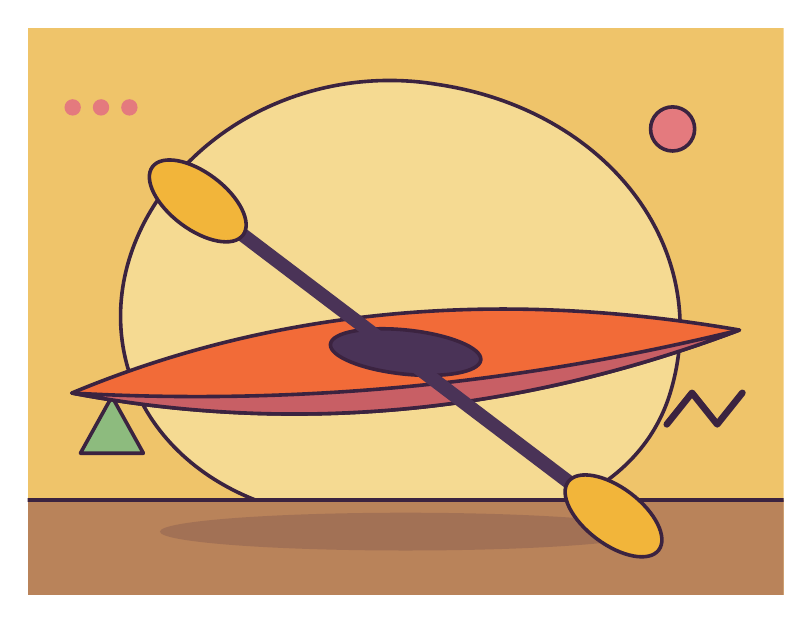
\begin{tikzpicture}
\clip (0,0) rectangle (240,180);
% background: wall, floor, blob, confetti
\fill[sky] (0,0) rectangle (240,180);
\filldraw[inked,fill=skyhi] (130,18) .. controls (184,26) and (218,70) .. (204,116) .. controls (190,162) and (122,168) .. (78,152) .. controls (34,138) and (18,96) .. (38,60) .. controls (56,28) and (94,12) .. (130,18) -- cycle;
\filldraw[inked,fill=coral] (204.77,32.15) circle [radius=7];
\draw[ink, line width=2.4pt, line cap=round, line join=round] (202.92,125.94) -- (210.92,115.94) -- (218.92,125.94) -- (226.92,115.94);
\filldraw[inked,fill=sage] (16.75,135.11) -- (26.75,117.11) -- (36.75,135.11) -- cycle;
\foreach \dx in {0,9,18} \fill[coral] (14.29+\dx,25.31) circle [radius=2.6];
\fill[wood] (0,150) rectangle (240,180);
\draw[ink, line width=1.3pt, line cap=round, line join=round] (0,150) -- (240,150);
\fill[ink, opacity=0.18] (120,160) ellipse [x radius=78, y radius=6];
% the item
\filldraw[inked,fill=orange] (14,116) .. controls (78,89.33) and (148.67,82.67) .. (226,96) .. controls (155.33,122.67) and (84.67,129.33) .. (14,116) -- cycle;
\filldraw[inked,fill=coraldk] (14,116) .. controls (84.67,120) and (155.33,113.33) .. (226,96) .. controls (155.33,122.67) and (84.67,129.33) .. (14,116) -- cycle;
\filldraw[inked,fill=dark,rotate around={-6:(120,103)}] (120,103) ellipse [x radius=24, y radius=7];
\draw[dark, line width=5pt, line cap=round, line join=round] (58,58) -- (182,152);
\filldraw[inked,fill=gold,rotate around={-37:(54,55)}] (54,55) ellipse [x radius=18, y radius=9];
\filldraw[inked,fill=gold,rotate around={-37:(186,155)}] (186,155) ellipse [x radius=18, y radius=9];
\end{tikzpicture}
\end{document}
